\def\year{2022}\relax
%File: formatting-instructions-latex-2022.tex
%release 2022.1
\documentclass[letterpaper]{article} % DO NOT CHANGE THIS
\usepackage{aaai22}  % DO NOT CHANGE THIS
\usepackage{times}  % DO NOT CHANGE THIS
\usepackage{helvet}  % DO NOT CHANGE THIS
\usepackage{courier}  % DO NOT CHANGE THIS
\usepackage[hyphens]{url}  % DO NOT CHANGE THIS
\usepackage{graphicx} % DO NOT CHANGE THIS
\urlstyle{rm} % DO NOT CHANGE THIS
\def\UrlFont{\rm}  % DO NOT CHANGE THIS
\usepackage{natbib}  % DO NOT CHANGE THIS AND DO NOT ADD ANY OPTIONS TO IT
\usepackage{caption} % DO NOT CHANGE THIS AND DO NOT ADD ANY OPTIONS TO IT
\DeclareCaptionStyle{ruled}{labelfont=normalfont,labelsep=colon,strut=off} % DO NOT CHANGE THIS
\frenchspacing  % DO NOT CHANGE THIS
\setlength{\pdfpagewidth}{8.5in}  % DO NOT CHANGE THIS
\setlength{\pdfpageheight}{11in}  % DO NOT CHANGE THIS
%
% These are recommended to typeset algorithms but not required. See the subsubsection on algorithms. Remove them if you don't have algorithms in your paper.
\usepackage{algorithm}
\usepackage{algorithmic}

%
% These are are recommended to typeset listings but not required. See the subsubsection on listing. Remove this block if you don't have listings in your paper.
\usepackage{newfloat}
\usepackage{listings}
\lstset{%
	basicstyle={\footnotesize\ttfamily},% footnotesize acceptable for monospace
	numbers=left,numberstyle=\footnotesize,xleftmargin=2em,% show line numbers, remove this entire line if you don't want the numbers.
	aboveskip=0pt,belowskip=0pt,%
	showstringspaces=false,tabsize=2,breaklines=true}
\floatstyle{ruled}
\newfloat{listing}{tb}{lst}{}
\floatname{listing}{Listing}
%
%\nocopyright
%
% PDF Info Is REQUIRED.
% For /Title, write your title in Mixed Case.
% Don't use accents or commands. Retain the parentheses.
% For /Author, add all authors within the parentheses,
% separated by commas. No accents, special characters
% or commands are allowed.
% Keep the /TemplateVersion tag as is
\pdfinfo{
/Title (Ludus: An Optimization Framework to Balance Auto Battler Cards)
/Author (Anonymous)
/TemplateVersion (2022.1)
}
%/Author (Nathaniel Budijono, Phoebe Goldman, Jack Maloney, Joseph B. Mueller, Phillip Walker, Jack Ladwig, Richard G. Freedman)
% Alternate name: BaOBAB (Balance Optimizer with Benchmarks in Auto Battlers)

% DISALLOWED PACKAGES
% \usepackage{authblk} -- This package is specifically forbidden
% \usepackage{balance} -- This package is specifically forbidden
% \usepackage{color (if used in text)
% \usepackage{CJK} -- This package is specifically forbidden
% \usepackage{float} -- This package is specifically forbidden
% \usepackage{flushend} -- This package is specifically forbidden
% \usepackage{fontenc} -- This package is specifically forbidden
% \usepackage{fullpage} -- This package is specifically forbidden
% \usepackage{geometry} -- This package is specifically forbidden
% \usepackage{grffile} -- This package is specifically forbidden
% \usepackage{hyperref} -- This package is specifically forbidden
% \usepackage{navigator} -- This package is specifically forbidden
% (or any other package that embeds links such as navigator or hyperref)
% \indentfirst} -- This package is specifically forbidden
% \layout} -- This package is specifically forbidden
% \multicol} -- This package is specifically forbidden
% \nameref} -- This package is specifically forbidden
% \usepackage{savetrees} -- This package is specifically forbidden
% \usepackage{setspace} -- This package is specifically forbidden
% \usepackage{stfloats} -- This package is specifically forbidden
% \usepackage{tabu} -- This package is specifically forbidden
% \usepackage{titlesec} -- This package is specifically forbidden
% \usepackage{tocbibind} -- This package is specifically forbidden
% \usepackage{ulem} -- This package is specifically forbidden
% \usepackage{wrapfig} -- This package is specifically forbidden
% DISALLOWED COMMANDS
% \nocopyright -- Your paper will not be published if you use this command
% \addtolength -- This command may not be used
% \balance -- This command may not be used
% \baselinestretch -- Your paper will not be published if you use this command
% \clearpage -- No page breaks of any kind may be used for the final version of your paper
% \columnsep -- This command may not be used
% \newpage -- No page breaks of any kind may be used for the final version of your paper
% \pagebreak -- No page breaks of any kind may be used for the final version of your paperr
% \pagestyle -- This command may not be used
% \tiny -- This is not an acceptable font size.
% \vspace{- -- No negative value may be used in proximity of a caption, figure, table, section, subsection, subsubsection, or reference
% \vskip{- -- No negative value may be used to alter spacing above or below a caption, figure, table, section, subsection, subsubsection, or reference

\setcounter{secnumdepth}{2} %May be changed to 1 or 2 if section numbers are desired.

% The file aaai22.sty is the style file for AAAI Press
% proceedings, working notes, and technical reports.
%

% Title

% Your title must be in mixed case, not sentence case.
% That means all verbs (including short verbs like be, is, using,and go),
% nouns, adverbs, adjectives should be capitalized, including both words in hyphenated terms, while
% articles, conjunctions, and prepositions are lower case unless they
% directly follow a colon or long dash
%\iffalse
%Example, Multiple Authors, ->> remove \iffalse,\fi and place them surrounding AAAI title to use it
\title{{\sc Ludus}: An Optimization Framework to Balance Auto Battler Cards}
% Framework, No metric exploration, Optimizing (not just balance)
%%Finding the Balance: An Exploration of Metrics to Design Balanced Character Stats in Auto Battler Games
\author {
    Submission \# 40
\if{false}
    % Authors
    Nathaniel Budijono\equalcontrib,\textsuperscript{\rm 1}
    Phoebe Goldman\equalcontrib, \textsuperscript{\rm 2}
    Jack Maloney\equalcontrib, \textsuperscript{\rm 3} \\
    Joseph B. Mueller, \textsuperscript{\rm 4,5}
    Phillip Walker, \textsuperscript{\rm 5}
    Jack Ladwig, \textsuperscript{\rm 5}
    Richard G. Freedman \textsuperscript{\rm 5}
\fi
}
\affiliations {
\if{false}
    % Affiliations
    \textsuperscript{\rm 1} University of Minnesota Twin Cities\\
    \textsuperscript{\rm 2} New York University\\
    \textsuperscript{\rm 3} University of Wisconsin-Madison\\
    \textsuperscript{\rm 4} University of Minnesota\\
    \textsuperscript{\rm 5} SIFT\\
    budij001@umn.edu, phoebe.goldman@nyu.edu, jmaloney3@wisc.edu, jmueller@sift.net, pwalker@sift.net, jladwig@sift.net, rfreedman@sift.net
\fi
}
%\fi

% our custom commands
\newcommand{\newterm}[1]{\textit{#1}}
\newcommand{\etal}{et al.\ }

\begin{document}

\maketitle

\begin{abstract}
  Auto battlers are a recent genre of online deck-building games
  where players choose and arrange cards that then compete against
  other players' cards in fully-automated battles. As in other
  deck-building games, such as trading card games, designers must
  balance the cards to permit a wide variety of competitive
  strategies.  We present {\sc Ludus}, a framework that combines
  automated playtesting with global search to optimize parameters for
  each card that will assist designers in balancing new content.  We
  develop an approximation algorithm to reduce the playtesting needed
  during optimization.  To guide the global search, we define metrics
  characterizing the health of the metagame and explore their impacts
  on the results of the optimization process.  Our research focuses on
  an auto battler game we designed for AI research, but our
  approach is applicable to other auto battler games.
\end{abstract}
%Future work: Need to develop AI to play non-auto battler deck-building games in ways representative of the player base.

% \noindent Congratulations on having a paper selected for inclusion in an AAAI Press proceedings or technical report! This document details the requirements necessary to get your accepted paper published using PDF\LaTeX{}. If you are using Microsoft Word, instructions are provided in a different document. AAAI Press does not support any other formatting software.

% The instructions herein are provided as a general guide for experienced \LaTeX{} users. If you do not know how to use \LaTeX{}, please obtain assistance locally. AAAI cannot provide you with support and the accompanying style files are \textbf{not} guaranteed to work. If the results you obtain are not in accordance with the specifications you received, you must correct your source file to achieve the correct result.

% These instructions are generic. Consequently, they do not include specific dates, page charges, and so forth. Please consult your specific written conference instructions for details regarding your submission. Please review the entire document for specific instructions that might apply to your particular situation. All authors must comply with the following:

% \begin{itemize}
% \item You must use the 2022 AAAI Press \LaTeX{} style file and the aaai22.bst bibliography style files, which are located in the 2022 AAAI Author Kit (aaai22.sty, aaai22.bst).
% \item You must complete, sign, and return by the deadline the AAAI copyright form (unless directed by AAAI Press to use the AAAI Distribution License instead).
% \item You must read and format your paper source and PDF according to the formatting instructions for authors.
% \item You must submit your electronic files and abstract using our electronic submission form \textbf{on time.}
% \item You must pay any required page or formatting charges to AAAI Press so that they are received by the deadline.
% \item You must check your paper before submitting it, ensuring that it compiles without error, and complies with the guidelines found in the AAAI Author Kit.
% \end{itemize}

% \section{Copyright}
% All papers submitted for publication by AAAI Press must be accompanied by a valid signed copyright form. They must also contain the AAAI copyright notice at the bottom of the first page of the paper. There are no exceptions to these requirements. If you fail to provide us with a signed copyright form or disable the copyright notice, we will be unable to publish your paper. There are \textbf{no exceptions} to this policy. You will find a PDF version of the AAAI copyright form in the AAAI AuthorKit. Please see the specific instructions for your conference for submission details.

% \section{Formatting Requirements in Brief}
% We need source and PDF files that can be used in a variety of ways and can be output on a variety of devices. The design and appearance of the paper is strictly governed by the aaai style file (aaai22.sty).
% \textbf{You must not make any changes to the aaai style file, nor use any commands, packages, style files, or macros within your own paper that alter that design, including, but not limited to spacing, floats, margins, fonts, font size, and appearance.} AAAI imposes requirements on your source and PDF files that must be followed. Most of these requirements are based on our efforts to standardize conference manuscript properties and layout. All papers submitted to AAAI for publication will be recompiled for standardization purposes. Consequently, every paper submission must comply with the following requirements:

% \begin{itemize}
% \item Your .tex file must compile in PDF\LaTeX{} --- (you may not include .ps or .eps figure files.)
% \item All fonts must be embedded in the PDF file --- including your figures.
% \item Modifications to the style file, whether directly or via commands in your document may not ever be made, most especially when made in an effort to avoid extra page charges or make your paper fit in a specific number of pages.
% \item No type 3 fonts may be used (even in illustrations).
% \item You may not alter the spacing above and below captions, figures, headings, and subheadings.
% \item You may not alter the font sizes of text elements, footnotes, heading elements, captions, or title information (for references and mathematics, please see the limited exceptions provided herein).
% \item You may not alter the line spacing of text.
% \item Your title must follow Title Case capitalization rules (not sentence case).
% \item Your .tex file must include completed metadata to pass-through to the PDF (see PDFINFO below).
% \item \LaTeX{} documents must use the Times or Nimbus font package (you may not use Computer Modern for the text of your paper).
% \item No \LaTeX{} 209 documents may be used or submitted.
% \item Your source must not require use of fonts for non-Roman alphabets within the text itself. If your paper includes symbols in other languages (such as, but not limited to, Arabic, Chinese, Hebrew, Japanese, Thai, Russian and other Cyrillic languages), you must restrict their use to bit-mapped figures. Fonts that require non-English language support (CID and Identity-H) must be converted to outlines or 300 dpi bitmap or removed from the document (even if they are in a graphics file embedded in the document).
% \item Two-column format in AAAI style is required for all papers.
% \item The paper size for final submission must be US letter without exception.
% \item The source file must exactly match the PDF.
% \item The document margins may not be exceeded (no overfull boxes).
% \item The number of pages and the file size must be as specified for your event.
% \item No document may be password protected.
% \item Neither the PDFs nor the source may contain any embedded links or bookmarks (no hyperref or navigator packages).
% \item Your source and PDF must not have any page numbers, footers, or headers (no pagestyle commands).
% \item Your PDF must be compatible with Acrobat 5 or higher.
% \item Your \LaTeX{} source file (excluding references) must consist of a \textbf{single} file (use of the ``input" command is not allowed.
% \item Your graphics must be sized appropriately outside of \LaTeX{} (do not use the ``clip" or ``trim'' command) .
% \end{itemize}

% If you do not follow these requirements, your paper will be returned to you to correct the deficiencies.

% \section{What Files to Submit}
% You must submit the following items to ensure that your paper is published:
% \begin{itemize}
% \item A fully-compliant PDF file that includes PDF metadata.
% \item Your \LaTeX{} source file submitted as a \textbf{single} .tex file (do not use the ``input" command to include sections of your paper --- every section must be in the single source file). (The only allowable exception is .bib file, which should be included separately).
% \item The bibliography (.bib) file(s).
% \item Your source must compile on our system, which includes only standard \LaTeX{} 2020 TeXLive support files.
% \item Only the graphics files used in compiling paper.
% \item The \LaTeX{}-generated files (e.g. .aux,  .bbl file, PDF, etc.).
% \end{itemize}

% Your \LaTeX{} source will be reviewed and recompiled on our system (if it does not compile, your paper will be returned to you. \textbf{Do not submit your source in multiple text files.} Your single \LaTeX{} source file must include all your text, your bibliography (formatted using aaai22.bst), and any custom macros.

% Your files should work without any supporting files (other than the program itself) on any computer with a standard \LaTeX{} distribution.

% \textbf{Do not send files that are not actually used in the paper.} We don't want you to send us any files not needed for compiling your paper, including, for example, this instructions file, unused graphics files, style files, additional material sent for the purpose of the paper review, and so forth.

% \textbf{Do not send supporting files that are not actually used in the paper.} We don't want you to send us any files not needed for compiling your paper, including, for example, this instructions file, unused graphics files, style files, additional material sent for the purpose of the paper review, and so forth.

% \textbf{Obsolete style files.} The commands for some common packages (such as some used for algorithms), may have changed. Please be certain that you are not compiling your paper using old or obsolete style files.

% \textbf{Final Archive.} Place your PDF and source files in a single archive which should be compressed using .zip. The final file size may not exceed 10 MB.
% Name your source file with the last (family) name of the first author, even if that is not you.


% \section{Using \LaTeX{} to Format Your Paper}

% The latest version of the AAAI style file is available on AAAI's website. Download this file and place it in the \TeX\ search path. Placing it in the same directory as the paper should also work. You must download the latest version of the complete AAAI Author Kit so that you will have the latest instruction set and style file.

% \subsection{Document Preamble}

% In the \LaTeX{} source for your paper, you \textbf{must} place the following lines as shown in the example in this subsection. This command set-up is for three authors. Add or subtract author and address lines as necessary, and uncomment the portions that apply to you. In most instances, this is all you need to do to format your paper in the Times font. The helvet package will cause Helvetica to be used for sans serif. These files are part of the PSNFSS2e package, which is freely available from many Internet sites (and is often part of a standard installation).

% Leave the setcounter for section number depth commented out and set at 0 unless you want to add section numbers to your paper. If you do add section numbers, you must uncomment this line and change the number to 1 (for section numbers), or 2 (for section and subsection numbers). The style file will not work properly with numbering of subsubsections, so do not use a number higher than 2.

% \subsubsection{The Following Must Appear in Your Preamble}
% \begin{quote}
% \begin{scriptsize}\begin{verbatim}
% \def\year{2022}\relax
% \documentclass[letterpaper]{article}
% % DO NOT CHANGE THIS
% \usepackage{aaai22} % DO NOT CHANGE THIS
% \usepackage{times} % DO NOT CHANGE THIS
% \usepackage{helvet} % DO NOT CHANGE THIS
% \usepackage{courier} % DO NOT CHANGE THIS
% \usepackage[hyphens]{url} % DO NOT CHANGE THIS
% \usepackage{graphicx} % DO NOT CHANGE THIS
% \urlstyle{rm} % DO NOT CHANGE THIS
% \def\UrlFont{\rm} % DO NOT CHANGE THIS
% \usepackage{graphicx}  % DO NOT CHANGE THIS
% \usepackage{natbib}  % DO NOT CHANGE THIS
% \usepackage{caption}  % DO NOT CHANGE THIS
% \DeclareCaptionStyle{ruled}%
%   {labelfont=normalfont,labelsep=colon,strut=off}
% \frenchspacing % DO NOT CHANGE THIS
% \setlength{\pdfpagewidth}{8.5in} % DO NOT CHANGE THIS
% \setlength{\pdfpageheight}{11in} % DO NOT CHANGE THIS
% %
% % PDF Info Is REQUIRED.
% % For /Title, write your title in Mixed Case.
% % Don't use accents or commands. Retain the parentheses.
% % For /Author, add all authors within the parentheses,
% % separated by commas. No accents, special characters
% % or commands are allowed.
% % Keep the /TemplateVersion tag as is
% \pdfinfo{
% /Title (AAAI Press Formatting Instructions for Authors
% Using LaTeX -- A Guide)
% /Author (AAAI Press Staff, Pater Patel Schneider,
% Sunil Issar, J. Scott Penberthy, George Ferguson,
% Hans Guesgen, Francisco Cruz, Marc Pujol-Gonzalez)
% /TemplateVersion (2022.1)
% }
% \end{verbatim}\end{scriptsize}
% \end{quote}

% \subsection{Preparing Your Paper}

% After the preamble above, you should prepare your paper as follows:
% \begin{quote}
% \begin{scriptsize}\begin{verbatim}
% \begin{document}
% \maketitle
% \begin{abstract}
% %...
% \end{abstract}\end{verbatim}\end{scriptsize}
% \end{quote}

% \noindent You should then continue with the body of your paper. Your paper must conclude with the references, which should be inserted as follows:
% \begin{quote}
% \begin{scriptsize}\begin{verbatim}
% % References and End of Paper
% % These lines must be placed at the end of your paper
% \bibliography{Bibliography-File}
% \end{document}
% \end{verbatim}\end{scriptsize}
% \end{quote}

% \subsection{Inserting Document Metadata with \LaTeX{}}
% PDF files contain document summary information that enables us to create an Acrobat index (pdx) file, and also allows search engines to locate and present your paper more accurately. \textit{Document metadata for author and title are REQUIRED.} You may not apply any script or macro to the implementation of the title, author, and metadata information in your paper.

% \textit{Important:} Do not include \textit{any} \LaTeX{} code or nonascii characters (including accented characters) in the metadata. The data in the metadata must be completely plain ascii. It may not include slashes, accents, linebreaks, unicode, or any \LaTeX{} commands. Type the title exactly as it appears on the paper (minus all formatting). Input the author names in the order in which they appear on the paper (minus all accents), separating each author by a comma. You may also include keywords in the optional Keywords field.

% \begin{quote}
% \begin{scriptsize}\begin{verbatim}
% \begin{document}\\
% \maketitle\\
% ...\\
% \bibliography{Bibliography-File}\\
% \end{document}\\
% \end{verbatim}\end{scriptsize}
% \end{quote}

% \subsection{Commands and Packages That May Not Be Used}
% \begin{table*}[t]
% \centering

% \begin{tabular}{l|l|l|l}
% \textbackslash abovecaption &
% \textbackslash abovedisplay &
% \textbackslash addevensidemargin &
% \textbackslash addsidemargin \\
% \textbackslash addtolength &
% \textbackslash baselinestretch &
% \textbackslash belowcaption &
% \textbackslash belowdisplay \\
% \textbackslash break &
% \textbackslash clearpage &
% \textbackslash clip &
% \textbackslash columnsep \\
% \textbackslash float &
% \textbackslash input &
% \textbackslash input &
% \textbackslash linespread \\
% \textbackslash newpage &
% \textbackslash pagebreak &
% \textbackslash renewcommand &
% \textbackslash setlength \\
% \textbackslash text height &
% \textbackslash tiny &
% \textbackslash top margin &
% \textbackslash trim \\
% \textbackslash vskip\{- &
% \textbackslash vspace\{- \\
% \end{tabular}
% %}
% \caption{Commands that must not be used}
% \label{table1}
% \end{table*}

% \begin{table}[t]
% \centering
% %\resizebox{.95\columnwidth}{!}{
% \begin{tabular}{l|l|l|l}
%     authblk & babel & cjk & dvips \\
%     epsf & epsfig & euler & float \\
%     fullpage & geometry & graphics & hyperref \\
%     layout & linespread & lmodern & maltepaper \\
%     navigator & pdfcomment & pgfplots & psfig \\
%     pstricks & t1enc & titlesec & tocbind \\
%     ulem
% \end{tabular}
% \caption{LaTeX style packages that must not be used.}
% \label{table2}
% \end{table}

% There are a number of packages, commands, scripts, and macros that are incompatable with aaai22.sty. The common ones are listed in tables \ref{table1} and \ref{table2}. Generally, if a command, package, script, or macro alters floats, margins, fonts, sizing, linespacing, or the presentation of the references and citations, it is unacceptable. Note that negative vskip and vspace may not be used except in certain rare occurances, and may never be used around tables, figures, captions, sections, subsections, subsubsections, or references.


% \subsection{Page Breaks}
% For your final camera ready copy, you must not use any page break commands. References must flow directly after the text without breaks. Note that some conferences require references to be on a separate page during the review process. AAAI Press, however, does not require this condition for the final paper.


% \subsection{Paper Size, Margins, and Column Width}
% Papers must be formatted to print in two-column format on 8.5 x 11 inch US letter-sized paper. The margins must be exactly as follows:
% \begin{itemize}
% \item Top margin: .75 inches
% \item Left margin: .75 inches
% \item Right margin: .75 inches
% \item Bottom margin: 1.25 inches
% \end{itemize}


% The default paper size in most installations of \LaTeX{} is A4. However, because we require that your electronic paper be formatted in US letter size, the preamble we have provided includes commands that alter the default to US letter size. Please note that using any other package to alter page size (such as, but not limited to the Geometry package) will result in your final paper being returned to you for correction.


% \subsubsection{Column Width and Margins.}
% To ensure maximum readability, your paper must include two columns. Each column should be 3.3 inches wide (slightly more than 3.25 inches), with a .375 inch (.952 cm) gutter of white space between the two columns. The aaai22.sty file will automatically create these columns for you.

% \subsection{Overlength Papers}
% If your paper is too long and you resort to formatting tricks to make it fit, it is quite likely that it will be returned to you. The best way to retain readability if the paper is overlength is to cut text, figures, or tables. There are a few acceptable ways to reduce paper size that don't affect readability. First, turn on \textbackslash frenchspacing, which will reduce the space after periods. Next, move all your figures and tables to the top of the page. Consider removing less important portions of a figure. If you use \textbackslash centering instead of \textbackslash begin\{center\} in your figure environment, you can also buy some space. For mathematical environments, you may reduce fontsize {\bf but not below 6.5 point}.


% Commands that alter page layout are forbidden. These include \textbackslash columnsep,  \textbackslash float, \textbackslash topmargin, \textbackslash topskip, \textbackslash textheight, \textbackslash textwidth, \textbackslash oddsidemargin, and \textbackslash evensizemargin (this list is not exhaustive). If you alter page layout, you will be required to pay the page fee. Other commands that are questionable and may cause your paper to be rejected include \textbackslash parindent, and \textbackslash parskip. Commands that alter the space between sections are forbidden. The title sec package is not allowed. Regardless of the above, if your paper is obviously ``squeezed" it is not going to to be accepted. Options for reducing the length of a paper include reducing the size of your graphics, cutting text, or paying the extra page charge (if it is offered).


% \subsection{Type Font and Size}
% Your paper must be formatted in Times Roman or Nimbus. We will not accept papers formatted using Computer Modern or Palatino or some other font as the text or heading typeface. Sans serif, when used, should be Courier. Use Symbol or Lucida or Computer Modern for \textit{mathematics only. }

% Do not use type 3 fonts for any portion of your paper, including graphics. Type 3 bitmapped fonts are designed for fixed resolution printers. Most print at 300 dpi even if the printer resolution is 1200 dpi or higher. They also often cause high resolution imagesetter devices to crash. Consequently, AAAI will not accept electronic files containing obsolete type 3 fonts. Files containing those fonts (even in graphics) will be rejected. (Authors using blackboard symbols must be avoid those packages that use type 3 fonts.)

% Fortunately, there are effective workarounds that will prevent your file from embedding type 3 bitmapped fonts. The easiest workaround is to use the required times, helvet, and courier packages with \LaTeX{}2e. (Note that papers formatted in this way will still use Computer Modern for the mathematics. To make the math look good, you'll either have to use Symbol or Lucida, or you will need to install type 1 Computer Modern fonts --- for more on these fonts, see the section ``Obtaining Type 1 Computer Modern.")

% If you are unsure if your paper contains type 3 fonts, view the PDF in Acrobat Reader. The Properties/Fonts window will display the font name, font type, and encoding properties of all the fonts in the document. If you are unsure if your graphics contain type 3 fonts (and they are PostScript or encapsulated PostScript documents), create PDF versions of them, and consult the properties window in Acrobat Reader.

% The default size for your type must be ten-point with twelve-point leading (line spacing). Start all pages (except the first) directly under the top margin. (See the next section for instructions on formatting the title page.) Indent ten points when beginning a new paragraph, unless the paragraph begins directly below a heading or subheading.


% \subsubsection{Obtaining Type 1 Computer Modern for \LaTeX{}.}

% If you use Computer Modern for the mathematics in your paper (you cannot use it for the text) you may need to download type 1 Computer fonts. They are available without charge from the American Mathematical Society:
% http://www.ams.org/tex/type1-fonts.html.

% \subsubsection{Nonroman Fonts.}
% If your paper includes symbols in other languages (such as, but not limited to, Arabic, Chinese, Hebrew, Japanese, Thai, Russian and other Cyrillic languages), you must restrict their use to bit-mapped figures.

% \subsection{Title and Authors}
% Your title must appear in mixed case (nouns, pronouns, and verbs are capitalized) near the top of the first page, centered over both columns in sixteen-point bold type (twenty-four point leading). This style is called ``mixed case" (or ``title case"), which means that all verbs (including short verbs like be, is, using, and go), nouns, adverbs, adjectives, and pronouns should be capitalized, (including both words in hyphenated terms), while articles, conjunctions, and prepositions are lower case unless they directly follow a colon or long dash.

% Author's names should appear below the title of the paper, centered in twelve-point type (with fifteen point leading), along with affiliation(s) and complete address(es) (including electronic mail address if available) in nine-point roman type (the twelve point leading). You should begin the two-column format when you come to the abstract.

% \subsubsection{Formatting Author Information.}
% Author information has to be set according the following specification depending if you have one or more than one affiliation.  You may not use a table nor may you employ the \textbackslash authorblk.sty package. For one or several authors from the same institution, please just separate with commas and write the affiliation directly below using the macros \textbackslash author and \textbackslash affiliations:

% \begin{quote}\begin{scriptsize}\begin{verbatim}
% \author{
%     Author 1, ..., Author n\\
% }
% \affiliations {
%     Address line\\
%     ... \\
%     Address line\\
% }
% \end{verbatim}\end{scriptsize}\end{quote}


% \noindent For authors from different institutions, use \textbackslash textsuperscript \{\textbackslash rm x \} to match authors and affiliations. Notice that there should not be any spaces between the author name (or comma following it) and the superscript.

% \begin{quote}\begin{scriptsize}\begin{verbatim}
% \author{
%     AuthorOne,\equalcontrib\textsuperscript{\rm 1}
%     AuthorTwo,\equalcontrib\textsuperscript{\rm 2}
%     AuthorThree,\textsuperscript{\rm 3}\\
%     AuthorFour,\textsuperscript{\rm 4}
%     AuthorFive \textsuperscript{\rm 5}}
% }
% \affiliations {
%     \textsuperscript{\rm 1}AffiliationOne,\\
%     \textsuperscript{\rm 2}AffiliationTwo,\\
%     \textsuperscript{\rm 3}AffiliationThree,\\
%     \textsuperscript{\rm 4}AffiliationFour,\\
%     \textsuperscript{\rm 5}AffiliationFive\\
%     \{email, email\}@affiliation.com,
%     email@affiliation.com,
%     email@affiliation.com,
%     email@affiliation.com
% }
% \end{verbatim}\end{scriptsize}\end{quote}

% You can indicate that some authors contributed equally using the \textbackslash equalcontrib command. This will add a marker after the author names and a footnote on the first page.

% Note that you may want to  break the author list for better visualization. You can achieve this using a simple line break (\textbackslash  \textbackslash).

% \subsection{\LaTeX{} Copyright Notice}
% The copyright notice automatically appears if you use aaai22.sty. It has been hardcoded and may not be disabled.

% \subsection{Credits}
% Any credits to a sponsoring agency should appear in the acknowledgments section, unless the agency requires different placement. If it is necessary to include this information on the front page, use
% \textbackslash thanks in either the \textbackslash author or \textbackslash title commands.
% For example:
% \begin{quote}
% \begin{small}
% \textbackslash title\{Very Important Results in AI\textbackslash thanks\{This work is
%  supported by everybody.\}\}
% \end{small}
% \end{quote}
% Multiple \textbackslash thanks commands can be given. Each will result in a separate footnote indication in the author or title with the corresponding text at the botton of the first column of the document. Note that the \textbackslash thanks command is fragile. You will need to use \textbackslash protect.

% Please do not include \textbackslash pubnote commands in your document.

% \subsection{Abstract}
% Follow the example commands in this document for creation of your abstract. The command \textbackslash begin\{abstract\} will automatically indent the text block. Please do not indent it further. {Do not include references in your abstract!}

% \subsection{Page Numbers}

% Do not \textbf{ever} print any page numbers on your paper. The use of \textbackslash pagestyle is forbidden.

% \subsection{Text }
% The main body of the paper must be formatted in black, ten-point Times Roman with twelve-point leading (line spacing). You may not reduce font size or the linespacing. Commands that alter font size or line spacing (including, but not limited to baselinestretch, baselineshift, linespread, and others) are expressly forbidden. In addition, you may not use color in the text.

% \subsection{Citations}
% Citations within the text should include the author's last name and year, for example (Newell 1980). Append lower-case letters to the year in cases of ambiguity. Multiple authors should be treated as follows: (Feigenbaum and Engelmore 1988) or (Ford, Hayes, and Glymour 1992). In the case of four or more authors, list only the first author, followed by et al. (Ford et al. 1997).

% \subsection{Extracts}
% Long quotations and extracts should be indented ten points from the left and right margins.

% \begin{quote}
% This is an example of an extract or quotation. Note the indent on both sides. Quotation marks are not necessary if you offset the text in a block like this, and properly identify and cite the quotation in the text.

% \end{quote}

% \subsection{Footnotes}
% Avoid footnotes as much as possible; they interrupt the reading of the text. When essential, they should be consecutively numbered throughout with superscript Arabic numbers. Footnotes should appear at the bottom of the page, separated from the text by a blank line space and a thin, half-point rule.

% \subsection{Headings and Sections}
% When necessary, headings should be used to separate major sections of your paper. Remember, you are writing a short paper, not a lengthy book! An overabundance of headings will tend to make your paper look more like an outline than a paper. The aaai22.sty package will create headings for you. Do not alter their size nor their spacing above or below.

% \subsubsection{Section Numbers.}
% The use of section numbers in AAAI Press papers is optional. To use section numbers in \LaTeX{}, uncomment the setcounter line in your document preamble and change the 0 to a 1. Section numbers should not be used in short poster papers and/or extended abstracts.

% \subsubsection{Section Headings.}
% Sections should be arranged and headed as follows:
% \begin{enumerate}
% \item Main content sections
% \item Appendices (optional)
% \item Ethical statement (optional, unnumbered)
% \item Acknowledgements (optional, unnumbered)
% \item References (unnumbered)
% \end{enumerate}

% \subsubsection{Appendices.}
% Any appendices must appear after the main content. If your main sections are numbered, appendix sections must use letters instead of arabic numerals. In \LaTeX{} you can use the \texttt{\textbackslash appendix} command to achieve this effect and then use \texttt{\textbackslash section\{Heading\}} normally for your appendix sections.

% \subsubsection{Ethical statement.}
% You can write a statement about the potential ethical impact of your work, including its broad societal implications, both positive and negative. If included, such statement must be written in an unnumbered section titled \emph{Ethical statement}.

% \subsubsection{Acknowledgments.}
% The acknowledgments section, if included, appears right before the references and is headed ``Acknowledgments". It must not be numbered even if other sections are (use \texttt{\textbackslash section*\{Acknowledgements\}} in \LaTeX{}). This section includes acknowledgments of help from associates and colleagues, credits to sponsoring agencies, financial support, and permission to publish. Please acknowledge other contributors, grant support, and so forth, in this section. Do not put acknowledgments in a footnote on the first page. If your grant agency requires acknowledgment of the grant on page 1, limit the footnote to the required statement, and put the remaining acknowledgments at the back. Please try to limit acknowledgments to no more than three sentences.

% \subsubsection{References.}
% The references section should be labeled ``References" and must appear at the very end of the paper (don't end the paper with references, and then put a figure by itself on the last page). A sample list of references is given later on in these instructions. Please use a consistent format for references. Poorly prepared or sloppy references reflect badly on the quality of your paper and your research. Please prepare complete and accurate citations.

% \subsection{Illustrations and  Figures}

% \begin{figure}[t]
% \centering
% %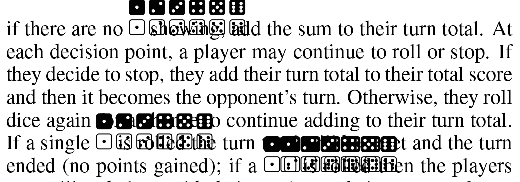
\includegraphics[width=0.9\columnwidth]{figure1} % Reduce the figure size so that it is slightly narrower than the column. Don't use precise values for figure width.This setup will avoid overfull boxes.
% \caption{Using the trim and clip commands produces fragile layers that can result in disasters (like this one from an actual paper) when the color space is corrected or the PDF combined with others for the final proceedings. Crop your figures properly in a graphics program -- not in LaTeX}.
% \label{fig1}
% \end{figure}

% \begin{figure*}[t]
% \centering
% %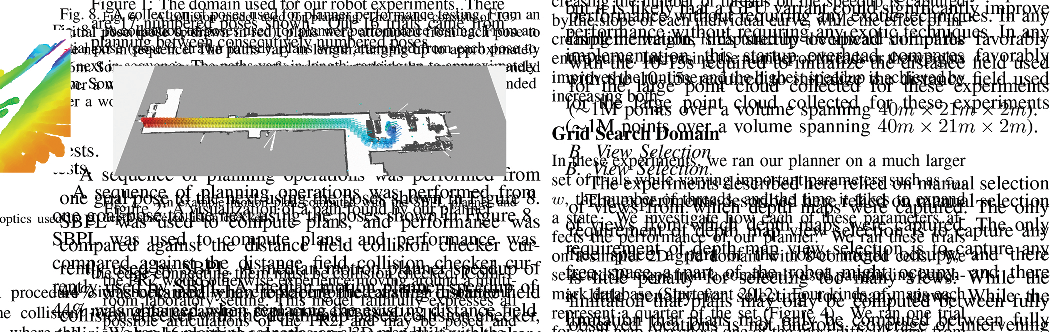
\includegraphics[width=0.8\textwidth]{figure2} % Reduce the figure size so that it is slightly narrower than the column.
% \caption{Adjusting the bounding box instead of actually removing the unwanted data resulted multiple layers in this paper. It also needlessly increased the PDF size. In this case, the size of the unwanted layer doubled the paper's size, and produced the following surprising results in final production. Crop your figures properly in a graphics program. Don't just alter the bounding box.}
% \label{fig2}
% \end{figure*}

% % Using the \centering command instead of \begin{center} ... \end{center} will save space
% % Positioning your figure at the top of the page will save space and make the paper more readable
% % Using 0.95\columnwidth in conjunction with the


% Your paper must compile in PDF\LaTeX{}. Consequently, all your figures must be .jpg, .png, or .pdf. You may not use the .gif (the resolution is too low), .ps, or .eps file format for your figures.

% Figures, drawings, tables, and photographs should be placed throughout the paper on the page (or the subsequent page) where they are first discussed. Do not group them together at the end of the paper. If placed at the top of the paper, illustrations may run across both columns. Figures must not invade the top, bottom, or side margin areas. Figures must be inserted using the \textbackslash usepackage\{graphicx\}. Number figures sequentially, for example, figure 1, and so on. Do not use minipage to group figures.

% If you normally create your figures using pgfplots, please create the figures first, and then import them as pdfs with proper bounding boxes, as the bounding and trim boxes created by pfgplots are fragile and not valid.

% When you include your figures, you must crop them \textbf{outside} of \LaTeX{}. The command \textbackslash includegraphics*[clip=true, viewport 0 0 10 10]{...} might result in a PDF that looks great, but the image is \textbf{not really cropped.} The full image can reappear (and obscure whatever it is overlapping) when page numbers are applied or color space is standardized. Figures \ref{fig1}, and \ref{fig2} display some unwanted results that often occur.

% If your paper includes illustrations that are not compatible with PDF\TeX{} (such as .eps or .ps documents), you will need to convert them. The epstopdf package will usually work for eps files. You will need to convert your ps files to PDF in either case.

% \subsubsection {Figure Captions.}The illustration number and caption must appear \textit{under} the illustration. Labels and other text with the actual illustration must be at least nine-point type. However, the font and size of figure captions must be 10 point roman. Do not make them smaller, bold, or italic. (Individual words may be italicized if the context requires differentiation.)

% \subsection{Tables}

% Tables should be presented in 10 point roman type. If necessary, they may be altered to 9 point type. You may not use any commands that further reduce point size below nine points. Tables that do not fit in a single column must be placed across double columns. If your table won't fit within the margins even when spanning both columns, you must split it. Do not use minipage to group tables.

% \subsubsection {Table Captions.} The number and caption for your table must appear \textit{under} (not above) the table.  Additionally, the font and size of table captions must be 10 point roman and must be placed beneath the figure. Do not make them smaller, bold, or italic. (Individual words may be italicized if the context requires differentiation.)



% \subsubsection{Low-Resolution Bitmaps.}
% You may not use low-resolution (such as 72 dpi) screen-dumps and GIF files---these files contain so few pixels that they are always blurry, and illegible when printed. If they are color, they will become an indecipherable mess when converted to black and white. This is always the case with gif files, which should never be used. The resolution of screen dumps can be increased by reducing the print size of the original file while retaining the same number of pixels. You can also enlarge files by manipulating them in software such as PhotoShop. Your figures should be 300 dpi when incorporated into your document.

% \subsubsection{\LaTeX{} Overflow.}
% \LaTeX{} users please beware: \LaTeX{} will sometimes put portions of the figure or table or an equation in the margin. If this happens, you need to make the figure or table span both columns. If absolutely necessary, you may reduce the figure, or reformat the equation, or reconfigure the table.{ \bf Check your log file!} You must fix any overflow into the margin (that means no overfull boxes in \LaTeX{}). \textbf{Nothing is permitted to intrude into the margin or gutter.}


% \subsubsection{Using Color.}
% Use of color is restricted to figures only. It must be WACG 2.0 compliant. (That is, the contrast ratio must be greater than 4.5:1 no matter the font size.) It must be CMYK, NOT RGB. It may never be used for any portion of the text of your paper. The archival version of your paper will be printed in black and white and grayscale. The web version must be readable by persons with disabilities. Consequently, because conversion to grayscale can cause undesirable effects (red changes to black, yellow can disappear, and so forth), we strongly suggest you avoid placing color figures in your document. If you do include color figures, you must (1) use the CMYK (not RGB) colorspace and (2) be mindful of readers who may happen to have trouble distinguishing colors. Your paper must be decipherable without using color for distinction.

% \subsubsection{Drawings.}
% We suggest you use computer drawing software (such as Adobe Illustrator or, (if unavoidable), the drawing tools in Microsoft Word) to create your illustrations. Do not use Microsoft Publisher. These illustrations will look best if all line widths are uniform (half- to two-point in size), and you do not create labels over shaded areas. Shading should be 133 lines per inch if possible. Use Times Roman or Helvetica for all figure call-outs. \textbf{Do not use hairline width lines} --- be sure that the stroke width of all lines is at least .5 pt. Zero point lines will print on a laser printer, but will completely disappear on the high-resolution devices used by our printers.

% \subsubsection{Photographs and Images.}
% Photographs and other images should be in grayscale (color photographs will not reproduce well; for example, red tones will reproduce as black, yellow may turn to white, and so forth) and set to a minimum of 300 dpi. Do not prescreen images.

% \subsubsection{Resizing Graphics.}
% Resize your graphics \textbf{before} you include them with LaTeX. You may \textbf{not} use trim or clip options as part of your \textbackslash includegraphics command. Resize the media box of your PDF using a graphics program instead.

% \subsubsection{Fonts in Your Illustrations.}
% You must embed all fonts in your graphics before including them in your LaTeX document.

% \subsubsection{Algorithms.}
% Algorithms and/or programs are a special kind of figures. Like all illustrations, they should appear floated to the top (preferably) or bottom of the page. However, their caption should appear in the header, left-justified and enclosed between horizontal lines, as shown in Algorithm~\ref{alg:algorithm}. The algorithm body should be terminated with another horizontal line. It is up to the authors to decide whether to show line numbers or not, how to format comments, etc.

% In \LaTeX{} algorithms may be typeset using the {\tt algorithm} and {\tt algorithmic} packages, but you can also use one of the many other packages for the task.

% \begin{algorithm}[tb]
% \caption{Example algorithm}
% \label{alg:algorithm}
% \textbf{Input}: Your algorithm's input\\
% \textbf{Parameter}: Optional list of parameters\\
% \textbf{Output}: Your algorithm's output
% \begin{algorithmic}[1] %[1] enables line numbers
% \STATE Let $t=0$.
% \WHILE{condition}
% \STATE Do some action.
% \IF {conditional}
% \STATE Perform task A.
% \ELSE
% \STATE Perform task B.
% \ENDIF
% \ENDWHILE
% \STATE \textbf{return} solution
% \end{algorithmic}
% \end{algorithm}

% \subsubsection{Listings.}
% Listings are much like algorithms and programs. They should also appear floated to the top (preferably) or bottom of the page. Listing captions should appear in the header, left-justified and enclosed between horizontal lines as shown in Listing~\ref{lst:listing}. Terminate the body with another horizontal line and avoid any background color. Line numbers, if included, must appear within the text column.

% \begin{listing}[tb]%
% \caption{Example listing {\tt quicksort.hs}}%
% \label{lst:listing}%
% \begin{lstlisting}[language=Haskell]
% quicksort :: Ord a => [a] -> [a]
% quicksort []     = []
% quicksort (p:xs) = (quicksort lesser) ++ [p] ++ (quicksort greater)
% 	where
% 		lesser  = filter (< p) xs
% 		greater = filter (>= p) xs
% \end{lstlisting}
% \end{listing}

% \subsection{References}
% The AAAI style includes a set of definitions for use in formatting references with BibTeX. These definitions make the bibliography style fairly close to the ones  specified in the Reference Examples appendix below. To use these definitions, you also need the BibTeX style file ``aaai22.bst," available in the AAAI Author Kit on the AAAI web site. Then, at the end of your paper but before \textbackslash end{document}, you need to put the following lines:

% \begin{quote}
% \begin{small}
% \textbackslash bibliography\{bibfile1,bibfile2,...\}
% \end{small}
% \end{quote}

% Please note that the aaai22.sty class already sets the bibliographystyle for you, so you do not have to place any \textbackslash bibliographystyle command in the document yourselves. The aaai22.sty file is incompatible with the hyperref and navigator packages. If you use either, your references will be garbled and your paper will be returned to you.

% References may be the same size as surrounding text. However, in this section (only), you may reduce the size to \textbackslash small if your paper exceeds the allowable number of pages. Making it any smaller than 9 point with 10 point linespacing, however, is not allowed. A more precise and exact method of reducing the size of your references minimally is by means of the following command: \begin{quote}
% \textbackslash fontsize\{9.8pt\}\{10.8pt\}
% \textbackslash selectfont\end{quote}

% \noindent You must reduce the size equally for both font size and line spacing, and may not reduce the size beyond \{9.0pt\}\{10.0pt\}.

% The list of files in the \textbackslash bibliography command should be the names of your BibTeX source files (that is, the .bib files referenced in your paper).

% The following commands are available for your use in citing references:
% \begin{quote}
% {\em \textbackslash cite:} Cites the given reference(s) with a full citation. This appears as ``(Author Year)'' for one reference, or ``(Author Year; Author Year)'' for multiple references.\smallskip\\
% {\em \textbackslash shortcite:} Cites the given reference(s) with just the year. This appears as ``(Year)'' for one reference, or ``(Year; Year)'' for multiple references.\smallskip\\
% {\em \textbackslash citeauthor:} Cites the given reference(s) with just the author name(s) and no parentheses.\smallskip\\
% {\em \textbackslash citeyear:} Cites the given reference(s) with just the date(s) and no parentheses.
% \end{quote}
% You may also use any of the \emph{natbib} citation commands.


% \section{Proofreading Your PDF}
% Please check all the pages of your PDF file. The most commonly forgotten element is the acknowledgements --- especially the correct grant number. Authors also commonly forget to add the metadata to the source, use the wrong reference style file, or don't follow the capitalization rules or comma placement for their author-title information properly. A final common problem is text (expecially equations) that runs into the margin. You will need to fix these common errors before submitting your file.

% \section{Improperly Formatted Files }
% In the past, AAAI has corrected improperly formatted files submitted by the authors. Unfortunately, this has become an increasingly burdensome expense that we can no longer absorb). Consequently, if your file is improperly formatted, it will be returned to you for correction.

% \subsection{\LaTeX{} 209 Warning}
% If you use \LaTeX{} 209 your paper will be returned to you unpublished. Convert your paper to \LaTeX{}2e.

% \section{Naming Your Electronic File}
% We require that you name your \LaTeX{} source file with the last name (family name) of the first author so that it can easily be differentiated from other submissions. Complete file-naming instructions will be provided to you in the submission instructions.

% \section{Submitting Your Electronic Files to AAAI}
% Instructions on paper submittal will be provided to you in your acceptance letter.

% \section{Inquiries}
% If you have any questions about the preparation or submission of your paper as instructed in this document, please contact AAAI Press at the address given below. If you have technical questions about implementation of the aaai style file, please contact an expert at your site. We do not provide technical support for \LaTeX{} or any other software package. To avoid problems, please keep your paper simple, and do not incorporate complicated macros and style files.

% \begin{quote}
% \noindent AAAI Press\\
% 2275 East Bayshore Road, Suite 160\\
% Palo Alto, California 94303\\
% \textit{Telephone:} (650) 328-3123\\
% \textit{E-mail:} See the submission instructions for your particular conference or event.
% \end{quote}

% \section{Additional Resources}
% \LaTeX{} is a difficult program to master. If you've used that software, and this document didn't help or some items were not explained clearly, we recommend you read Michael Shell's excellent document (testflow doc.txt V1.0a 2002/08/13) about obtaining correct PS/PDF output on \LaTeX{} systems. (It was written for another purpose, but it has general application as well). It is available at www.ctan.org in the tex-archive.

% \appendix
% \section{Reference Examples}
% \label{sec:reference_examples}

% \nobibliography*
% Formatted bibliographies should look like the following examples. You should use BibTeX to generate the references. Missing fields are unacceptable when compiling references, and usually indicate that you are using the wrong type of entry (BibTeX class).

% \paragraph{Book with multiple authors~\nocite{em:86}} Use the \texttt{@book} class.\\[.2em]
% \bibentry{em:86}.

% \paragraph{Journal and magazine articles~\nocite{r:80, hcr:83}} Use the \texttt{@article} class.\\[.2em]
% \bibentry{r:80}.\\[.2em]
% \bibentry{hcr:83}.

% \paragraph{Proceedings paper published by a society, press or publisher~\nocite{c:83, c:84}} Use the \texttt{@inproceedings} class. You may abbreviate the \emph{booktitle} field, but make sure that the conference edition is clear.\\[.2em]
% \bibentry{c:84}.\\[.2em]
% \bibentry{c:83}.

% \paragraph{University technical report~\nocite{r:86}} Use the \texttt{@techreport} class.\\[.2em]
% \bibentry{r:86}.

% \paragraph{Dissertation or thesis~\nocite{c:79}} Use the \texttt{@phdthesis} class.\\[.2em]
% \bibentry{c:79}.

% \paragraph{Forthcoming publication~\nocite{c:21}} Use the \texttt{@misc} class with a \texttt{note="Forthcoming"} annotation.
% \begin{quote}
% \begin{footnotesize}
% \begin{verbatim}
% @misc(key,
%   [...]
%   note="Forthcoming",
% )
% \end{verbatim}
% \end{footnotesize}
% \end{quote}
% \bibentry{c:21}.

% \paragraph{ArXiv paper~\nocite{c:22}} Fetch the BibTeX entry from the "Export Bibtex Citation" link in the arXiv website. Notice it uses the \texttt{@misc} class instead of the \texttt{@article} one, and that it includes the \texttt{eprint} and \texttt{archivePrefix} keys.
% \begin{quote}
% \begin{footnotesize}
% \begin{verbatim}
% @misc(key,
%   [...]
%   eprint="xxxx.yyyy",
%   archivePrefix="arXiv",
% )
% \end{verbatim}
% \end{footnotesize}
% \end{quote}
% \bibentry{c:22}.

% \paragraph{Website or online resource~\nocite{c:23}} Use the \texttt{@misc} class. Add the url in the \texttt{howpublished} field and the date of access in the \texttt{note} field:
% \begin{quote}
% \begin{footnotesize}
% \begin{verbatim}
% @misc(key,
%   [...]
%   howpublished="\url{http://...}",
%   note="Accessed: YYYY-mm-dd",
% )
% \end{verbatim}
% \end{footnotesize}
% \end{quote}
% \bibentry{c:23}.

% \vspace{.2em}
% For the most up to date version of the AAAI reference style, please consult the \textit{AI Magazine} Author Guidelines at \url{https://aaai.org/ojs/index.php/aimagazine/about/submissions#authorGuidelines}

% % Use \bibliography{yourbibfile} instead or the References section will not appear in your paper
% \nobibliography{aaai22}

% \section{Acknowledgments}
% AAAI is especially grateful to Peter Patel Schneider for his work in implementing the original aaai.sty file, liberally using the ideas of other style hackers, including Barbara Beeton. We also acknowledge with thanks the work of George Ferguson for his guide to using the style and BibTeX files --- which has been incorporated into this document --- and Hans Guesgen, who provided several timely modifications, as well as the many others who have, from time to time, sent in suggestions on improvements to the AAAI style. We are especially grateful to Francisco Cruz, Marc Pujol-Gonzalez, and Mico Loretan for the improvements to the Bib\TeX{} and \LaTeX{} files made in 2020.

% The preparation of the \LaTeX{} and Bib\TeX{} files that implement these instructions was supported by Schlumberger Palo Alto Research, AT\&T Bell Laboratories, Morgan Kaufmann Publishers, The Live Oak Press, LLC, and AAAI Press. Bibliography style changes were added by Sunil Issar. \verb+\+pubnote was added by J. Scott Penberthy. George Ferguson added support for printing the AAAI copyright slug. Additional changes to aaai22.sty and aaai22.bst have been made by Francisco Cruz, Marc Pujol-Gonzalez, and Mico Loretan.

% \bigskip
% \noindent Thank you for reading these instructions carefully. We look forward to receiving your electronic files!

\section{Introduction} \label{sec:introduction}
% I'm writing this intro to be read following the abstract.

Deck-building games are a genre of card games where each player
constructs a deck by combining cards from a heterogeneous pool, often
called a \newterm{set,} according to some \newterm{deck-building
  rules.} Players then \newterm{pilot} their decks in games against
other players' decks by strategically selecting which cards to play as
each unique game unfolds. Because it takes place prior to and effects
the outcomes of multiple individual games, the deck-building process
is often called the \newterm{metagame.}  Metagames are said to be
\newterm{healthy} when there are many diverse \enquote{archetypes}, or
categories of decks, available for players to choose between.
% FIXME: this clause is imprecise, & invites criticism re: "how do you
% measure how fun a game is"
% and when most games between these decks are fun.
% consider replacing with "enabling a wider array of strategic
% deck-building decisions and more varied, and therefore more
% interesting, individual games."
Deck-building games pose a challenge for game designers, since a
relatively small number of cards can be combined into a large number
of possible decks, which in turn can be paired into an even larger
number of match-ups. Human playtesting has repeatedly failed to
identify card designs or sets that lead to unhealthy metagames.
% TODO: do we need to cite sources?
% possible examples:
% - hearthstone's "miracle rogue" and "grim patron" metagames
% - magic: the gathering's "combo winter," "affinity," "caw-blade" and "oko" metagames
% - yu-gi-oh, i assume
% - to a lesser extent, "good boy" in storybook brawl
Even when it does successfully identify and fix unhealthy metagames,
human playtesting is often prohibitively expensive, requiring
significant labor and time from a number of skilled players. In this
paper, we attempt to reduce this cost by automating the balancing
process.
% this is where I cut off because I'm going to a movie.


\section{Methods} \label{sec:methods}
% shall we have a discussion section after methods and results?
% Discussion
% 	- possibility of using the "domination graph" as data,
% 	where decks are nodes and win rates are the directed
% 	edges
% 	- there is some correlation in the win rate dictionary
% 	distribution, as cards appear alongside other cards
% 	- we don't use a Hessian or Jacobian based opt method,
% 	which would have been useful to understand sensitivity

To achieve the goals outlined in the introduction, we built a simple auto-battler game. In this game we implemented a small number of special cards with extra mechanics, as well as a basic `vanilla' card that only engages in standard combat and has no extra mechanics. The details of these cards and their mechanics are explained below in Section~\ref{sec:ab-game-def}. The health and attack values of all cards can be adjusted, as well as some values pertaining to the extra mechanics (such as how much damage to deal to an opponent when a card dies). Multiple cards of the same type, but with different attack, health, or other values can be put into consideration in the same game. 

Beyond the auto-battler itself, we also constructed an optimization framework to find configurations of available cards which are balanced, fair, and fun. These criteria are obviously quite subjective, so new metrics are easily pluggable into the existing framework, as game designers develop new ways of capturing their goals and preferences about the metagame. A few simple options are explored within this paper as well.

\subsection{Playtesting simulator} \label{sec:sim}

To serve as a data source for quantitative analysis, we create
a playtesting simulator of a simplified auto battler game. 
This simulator is designed for research. It allows the user to 
create cards with new mechanics and run tournaments between
arbitrary decks. 

\subsubsection{Simplified game definition} \label{sec:ab-game-def}

Cards have nonnegative integer statistics including health points, 
attack, and parameters pertaining to a special mechanism. Such special parameters
developed include the following:

% consider table instead of bullets for space
\begin{itemize}
	\item Explosion damage. When the card dies, it damages
	each of the opponent's cards by this many health points.
	\item Heal amount. Prior to entering combat, the card 
	restores this many health points to its player's rightmost
	card
	\item Attack growth per hit. When the card takes damage, its
	attack increases by this many points.
	\item Explosion heal. When the card dies, it heals
	each of its player's other cards by this many health points.
	\item Heal donation percent. When the card would be healed,
	it instead restores this many percent of the health points
	to itself and donates the remaining health points to its
	player's other cards evenly.
	\item Armor points. The card starts with this many armor points.
	When the card would be damaged, it instead loses an armor point.
	When the card has zero armor points, it may be damaged normally.
	\item Damage split percent. When the card would be damaged,
	it instead receives this many percent of the damage to itself
	and splits the remaining damage evenly to its player's other cards.
	\item Middle age. Prior to entering combat, the card increases its
	attack by 1 if it has not participated in this many combat phases.
	After this many combat phases, the card decreases its attack by 1
	before entering combat.
	\item Target age. When the card dies, if it participated in this many
	combat phases, deal this many damage points to each of the opponent's
	cards. If the card participated in fewer than this many combat phases, 
	heal each of its player's other cards by health points equal to the
	number of combat phases in which the card participated.
	\item Detonation time. When the card has been healed or damaged this
	many times, the card and its opponent both die.
\end{itemize}

Other card mechanics without parameters include the ability to copy the 
attack of the opponent's cards (morphing enemies) and the ability to swap 
its health points and attack whenever its attack is greater than its health 
points (survivalist).

\subsubsection{Match procedure} \label{sec:game}

For the simulator, gameplay proceeds as follows:

\begin{enumerate}
	\item Each player in a tournament selects an ordered list
	of cards to be their deck.
	\item Prior to combat, the deck is arranged left-to-right.
	\item Each combat phase pits the leftmost surviving card
	of each player against each other. The cards take damage by 
	reducing their health points by their opponent card's attack.
	Cards with zero or fewer health points are dead. Surviving cards
	are arranged to be the rightmost card of their respective decks.
	\item Repeat combat until one or fewer players has a surviving card
	or the maximum number of combat phases allowed has been reached.
	If both or neither players have at least one surviving card, the game is a tie.
	Otherwise, the player with a surviving card wins.
\end{enumerate}

\subsubsection{Tournament procedure} \label{sec:tourney}

Over the course of a simulation, these matches are run within one of two types of tournaments:

\begin{enumerate}
	\item Round-robin tournament. Each deck plays one match against every other deck.
	For $n$ decks, this results in $n(n-1)/2 = n^2/2 - n/2 = O(n^2)$ matches.
	\item Group tournament. Due to the quadratic scalling of the number of matches in round-robin
	tournaments, they quickly become prohibitively large to simulate. Thus, we may want to sample from every possible 
	matchup in order to estimate the win rates of cards and decks. We do this by 
	partitioning the decks into groups of uniform size and running round-robin tournaments within these groups.
	For a group tournament with $k$ groups and $n$ total decks, this results in $k(n/k)(n/k - 1)/2 = n^2/(2k) - n/2$ matches in the case where 
	$n$ is divisible by $k$, which is the worst case in terms of number of matches.
\end{enumerate}

Combined with a metric measuring the health of the metagame, this simulator 
forms an approximation algorithm that estimates parity within the game.

\subsection{Metrics} \label{sec:metrics}

Quantitative measures of metagame health are needed to guide 
card statistic optimization. We present metrics built upon the
output data of the playtesting simulator described previously.

The playtesting simulation outputs a data vector $v$.
Each entry $v_i \in [-1, 1]$ represents the average payoff of
the deck at index $i$ during the last round of playtesting in
the optimization process. A payoff of 1 indicates a win. A
payoff of 0 means a tie, and a loss results in a payoff of -1.
The average of these payoffs over the course of the simulated
tournament for a deck make up the entries of $v$.

We then transform $v$ into another vector of length $n$ which maps a card to the
average win rate of the decks in which the card appears. This
vector $w$ has entries
$w_j \in [0, 1]$, the average win rate of the decks in which
the card at index $j$ appears. We present three metrics that 
use this distribution of win rates among the cards.

\subsubsection{Per-card payoff}

\begin{equation}
	\mathrm{PCP} = \frac{1}{n} \sum_j \left|\mathrm{payoff}(w_j)\right|^2
\end{equation}

Since average payoffs are equal to 0 when a deck when it wins as many matches as it loses, this is a metric to 
minimize if we want to punish very competitive or terrible decks.

\subsubsection{Standard deviation metric}

\begin{equation}
	\mathrm{SDM} = \sqrt{\frac{1}{n} \sum_j \left|w_j - \left(\frac{1}{n}\sum_j w_j\right)\right|^2}
\end{equation}

Standard deviation of the win rates is a metric we may seek to minimize. Doing so may avoid cards with
very high or low win rates compared to others.

\subsubsection{Entropy metric}

\begin{equation}
	\mathrm{EM} = -\sum_j \frac{w_j}{\sum_j w_j} \log\left(\frac{w_j}{\sum_j w_j}\right)
\end{equation}

Entropy of the win rates is a metric we may seek to maximize. When entropy is maximized, we approach a uniform
distribution of cards over win rates.

\subsubsection{Other metrics}

Our framework is flexible; researchers and designers alike may develop their own metrics corresponding to their
own ideas of what constitutes a healthy metagame. For example, a game designer may know from historical data that
a certain distribution of cards or decks over win rates corresponded to a period of celebrated parity in the metagame. 
The designer could conceivably use the Wasserstein distance or Kullback--Leibler 
divergence between this historical distribution and another distribution as a metric. Minimizing this metric 
might maintain similar levels of parity through future iterations of card releases.

\subsection{Optimization}

We use the \citeauthor{gad2021pygad}'s \shortcite{gad2021pygad} PyGAD python library for genetic optimization algorithms. This will attempt to find the optimal values of
parameters, which may include health points, attack, and special parameters, that optimizes
the chosen metric.

We constrain the genetic algorithm to consider integer values of the parameters between 1 and 10, inclusive. While hyperparameter tuning may have yielded better results,
we chose to run the genetic algorithm with 8 solutions and 4 parents mating per population for 32 generations in each experiment.

\subsection{Qualitative analysis}

Another way to understand the landscape of the metagame is through more qualitative methods. We look at two different ways of plotting data about the game results which give insights into the health and stability of the metagame. 

The first plot is a sweep over two variables, typically of the same card, although not necessarily. This gives a visual representation of the metagame throughout various configurations, and can lead to some interesting insights about the relationship between cards.

\begin{figure}[t]
	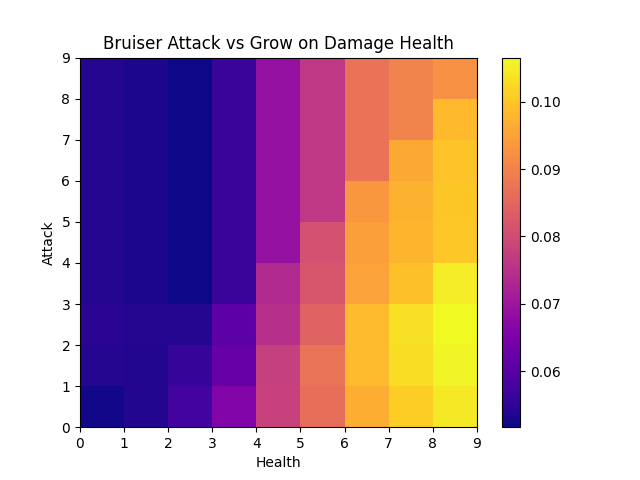
\includegraphics[width=10cm, height=8cm]{bruiser_vs_grow} 
	\caption{Plot of standard deviation metric for various values of the attack of a card with no special parameters fixed at 1 health point (bruiser) and the health points of a card with attack growth per hit and initial attack fixed at 1 (grow on damage)}
	\label{fig:bruiser_vs_grow}
\end{figure}

Take, for example, the plot in Figure~\ref{fig:bruiser_vs_grow}, of the value of the standard deviation metric given various values for the attack of the bruiser card and the health of the grow on damage card. The bruiser card is a vanilla card with a high attack (although variable in this situation) and one health point. The grow on damage card has a mechanic where each time it takes damage it gains one attack. Initially this card has no attack, and in this situation has a variable amount of health. If the grow on damage card is able to consistently become a powerful threat, it can become too strong, and a necessity for high level play, leading to an unbalanced metagame.

In the figure we can see that configurations in the upper left corner, where the attack of the bruiser is greater than the health of the grow on damage card, tend to be much more favorable than the configurations in the lower right corner, where the opposite is true. This evidence supports the intuitive idea that the bruiser's high attack is a good counter to the grow on damage card, because it can quickly remove the monster before it has had enough interactions to grow its damage to a large number. This kind of information can be quite useful to a game designer, who can see very clearly that the inclusion of a high damage card can improve the metagame dramatically if the grow on damage card is found to be too powerful.

The second plot explored is a histogram of the deck win rates. After running a tournament amongst all possible decks, the win rates of each deck are plotted in a histogram. The resulting distribution can have features which are indicative of the state of the health of metagame. For example, examine the difference between the distributions shown in Figure~\ref{fig:special_only_dist}. 

\begin{figure}[t]
	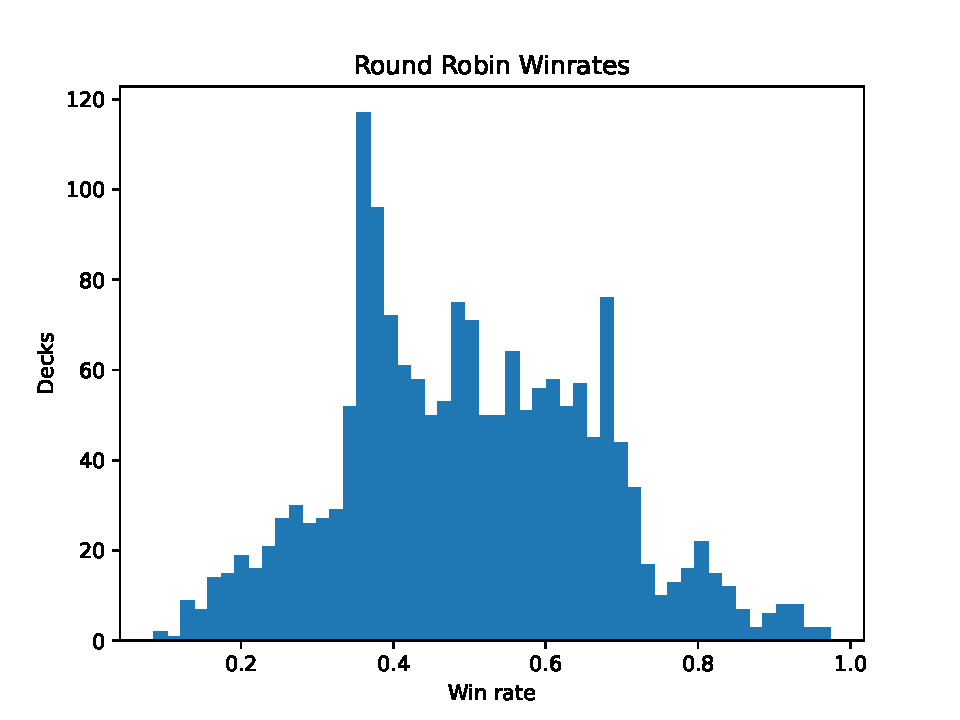
\includegraphics[width=4cm, height=4cm]{special_only_4_5_8_8_4_8_3_3_3_5}
	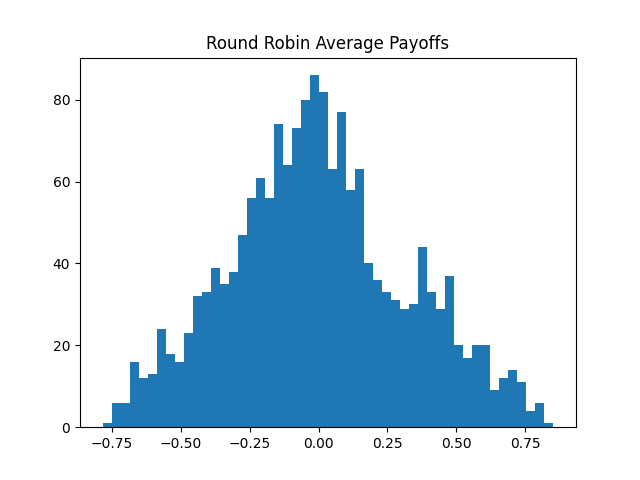
\includegraphics[width=4cm, height=4cm]{special_only_1_3_4_3_3_1_7_8_5_7}
	\caption{Distribution of win rates over decks in a poorly vs well balanced metagame}
	\label{fig:special_only_dist}
\end{figure}

In the first figure on the left we have a much wider and flatter distribution, where as in the one on the right, much more of the decks are centered around a 50\% win rate. 

\subsection{Experiment design}

% in methods: only describe the phases of experiments in a high level -- 1. build decks 2. tournaments 3. ... their common pattern
% describe set up, techniques; write about analysis and numbers in results

Our experiments share common phases.

\begin{enumerate}
	\item Build decks. We generate a set of cards and their associated attack, health points, and special parameters.
	Depending on the experiment, some or all of these variables may be varied from simulation to simulation during the optimization process.
	From this set of cards, the decks are permutations of 3 cards from the set, allowing for duplicates.
	\item Run tournaments. This will be either be a group or a round-robin tournament as described in Section~\ref{sec:tourney}.
	\item Optimize. These tournaments are run within each iteration of our genetic algorithm to produce a metric estimating the best
	possible health of the metagame with respect to parameters of the built decks.
\end{enumerate}


\section{Results} \label{sec:results}
\subsection{Group versus round-robin tournament}

% Maybe explain the group tournament in more detail
The first experiment we ran was to determine the efficacy of our sampling method. To do this, we compared the win rates of identical decks in a complete round robin tournament (every combination of decks played) with the win rate in a tournament conducted by randomly grouping decks into groups of various sizes, and then playing every combination of the decks within those groups.

\begin{figure}[t]
	\centering
	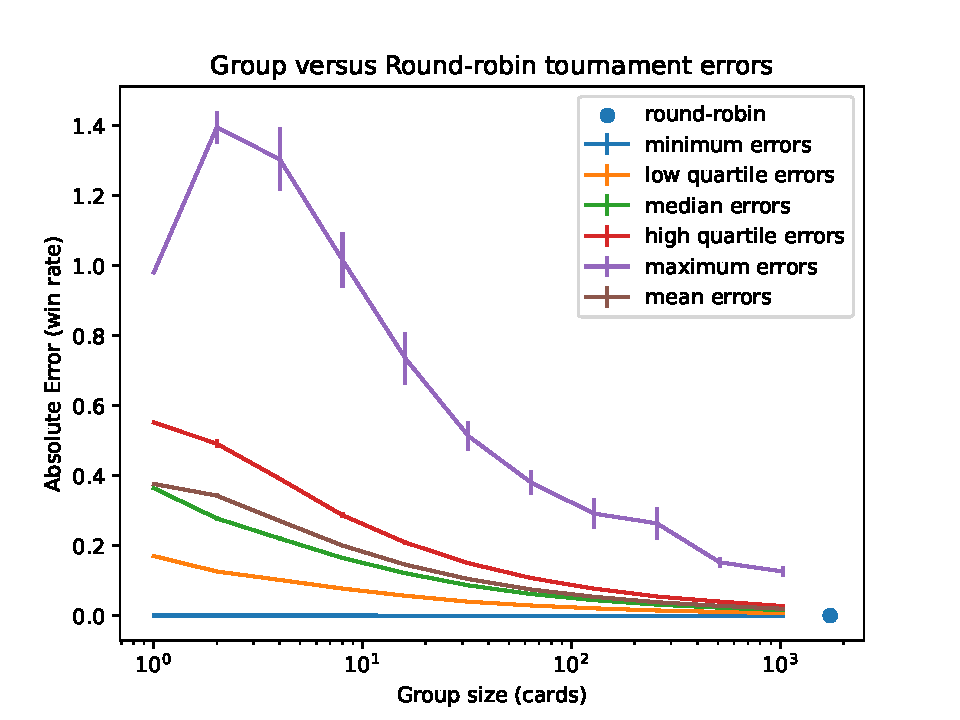
\includegraphics[width=0.9\columnwidth]{group_vs_rr_fig}
	\caption{Absolute value of the difference in win rate between a \textit{group tournament} of varying size and a full round-robin tournamnt of 1728 possible decks, along with error bars}
	\label{fig:group_vs_rr}
\end{figure}

%% Table

We then compute the average error over all of the decks, and we can see a steady convergence of the two values in Figure~\ref{fig:group_vs_rr}.

% Another table

 \subsection{Optimizing cards without special mechanisms}

The next experiment was to optimize a set of four basic cards, with no extra mechanics. We hypothesized that the `optimal' solution in terms of the standard deviation metric would be to have 4 identical cards, because then there would be only one card and thus zero standard deviation in the win rate of one card. We also recognized, however, that due to the limited number of generations run by our genetic algorithm, there was no guarantee it would find this solution. This case seemed even more interesting from a game design perspective, as a game with only a single card is obviously an uninteresting game, so we would like to see what `almost-optimal' solutions appear for this setup. This observation also illustrates a case where the standard deviation metric fails to fully capture the qualities we wish to optimize in our game.

The results of this experiment illustrate a different failure case of our standard deviation metric, one that had not been predicted. The genetic algorithm quickly found the solution (5/3), (5/4), (8/3), (8/1), where ($a$,$b$) indicates a card with $a$ attack and $b$ health points. This solution had zero standard deviation. Why? Any pairing of these cards will result in both cards being killed. Thus, every game ends after one round in a tie, and so there is no variance in win rates amongst the decks. 

 \subsection{Optimizing only special parameters}

The third experiment was to optimize a number of cards, each with a special mechanic. Each of these cards was assigned an intuitive value for it's attack and health, as a game designer might do. We then optimized the stats that controlled the special mechanics of these cards. We were interested to see how feasible it is to optimize the game with these constraints, and how impactful the special mechanics would be for the overall balance of the game. The cards used in this experiment are described in Table~\ref{tab:special_cards}.

\begin{table*}[t]
\centering
\begin{tabular}{||c c c c||} 
 \hline
 Card & Attack & Health & Variable special parameter (see Section~\ref{sec:ab-game-def})\\ [0.5ex] 
 \hline\hline
 Explode On Death & 2 & 1 & Damage dealt to enemies on death \\ 
 \hline
 Friendly Vampire & 1 & 3 & Amount of heath granted to ally \\
 \hline
 Grow On Damage & 0 & 5 & Attack gained per hit taken \\
 \hline
 Heal On Death & 1 & 2 & Health granted to allies on death \\
 \hline
 Health Donor & 1 & 4 & Percent of healing received that is split amongst allies \\
 \hline
 Ignore First Damage & 2 & 1 & Number of attacks which result in no damage taken \\
 \hline
 Morph Attack & 0 & 3 & N/A \\
 \hline
 Pain Splitter & 2 & 2 & Percent of damage taken that is split amongst allies \\
 \hline
 Rampage & 0 & 4 & Middle Age  \\
 \hline
 Survivalist & 2 & 2 & N/A \\
 \hline
 Threshold & 2 & 2 & Number of battles it must survive to damage all opponents on death \\
 \hline
 Time Bomb & 1 & 8 & Number of interactions before it will explode during the next battle \\ 
 \hline
\end{tabular}
\caption{Variable and set parameters for the \textit{optimize special parameters} experiment}
\label{tab:special_cards}
\end{table*}

The optimizer improved the win rate standard deviation from 0.0751 to 0.0589. 

\subsection{Optimizing health points, attack, and special parameters} \label{sec:first_set}

After fixing the attack and health, and focusing solely on the special mechanics, the next logical experiment is to tune both the attack and health, as well as the special mechanics. To reduce the huge dimensionality of this experiment we selected only five cards to optimize. They are listed in Table~\ref{tab:first_set}.

% First Set
\begin{table*}[t]
\centering
\begin{tabular}{||c c c c||} 
 \hline
 Card & Optimized Attack & Optimized Health & Optimized Variable Mechanic (see Section~\ref{sec:ab-game-def})\\ [0.5ex]
 \hline
 Survivalist &  &  & N/A \\
 \hline
 Morph Attack &  &  & N/A \\
 \hline
 Ignore First Damage &  &  & \\
 \hline
 Explode On Death &  &  &  \\ 
 \hline
 Vanilla &  &  &  \\
 \hline
\end{tabular}
\caption{List of cards in the first set, and their optimized solution}
\label{tab:first_set}
\end{table*}

The optimizer improved the win rate standard deviation from 0.0704 to 0.0584. This minimum is approximately the same as the one achieved in the previous experiment, modifying only the values of the special mechanics. One important observation, however, is that in both cases the optimizer was still making good progress in the final generations of our experiments. This indicates that these minima are not global, but that with further compute time and generations they could continue to improve.

\subsection{Optimizing after a set rotation}

Another common scenario encountered by designers of trading card games is that of releasing a new set or batch of cards, while maintaining the compatibility, fairness, and competitiveness of the previously released cards. To apply our toolset to this problem we first took the set of five cards and the optimized solution found in Section~\ref{sec:first_set}. This represents the first set of cards released. Next we selected another five cards, described in table Table~\ref{tab:second_set}, and optimized them, while keeping the values from the first set fixed at the solution found previously. 

% Compare this to the solution found by treating all 10 cards as one set

% Second Set
\begin{table*}[t]
\centering
\begin{tabular}{||c c c c||} 
 \hline
 Card & Optimized Attack & Optimized Health & Optimized Variable Mechanic (see Section~\ref{sec:ab-game-def})\\ [0.5ex]
 \hline
 Friendly Vampire &  &  &  \\
 \hline
 Grow On Damage &  &  &  \\
 \hline
 Heal On Death &  &  & \\
 \hline
 Rampage &  &  &  \\ 
 \hline
 Vanilla &  &  &  \\
 \hline
\end{tabular}
\caption{List of cards in the second set, and their optimized solution}
\label{tab:second_set}
\end{table*}

The optimizer improved the win rate standard deviation from 0.0591 to 0.0541. This is a comparatively smaller improvement than the previous experiments, however, the initial state is already in much better condition than either of the previous experiments. This is interesting, because it could indicate that adding new cards to an already well balanced set may not disturb the balance as much as one might expect. 


% \subsubsection{Optimizing an exhaustive round-robin tournament}


% write background and related work as a subsection?
\section{Related Works}
As the auto battler genre is still new, we were only able to find one other work
that specifically addresses the use of AI in their design.  \citeauthor{tencent_autobattle_lineup}
\shortcite{tencent_autobattle_lineup} focused on autonomously identifying the
best decks that players can construct given the available cards, game rules, and
decks that the game's designers expect to be played the most\footnote{Due to
Tencent's own game being the specific application, they use different terminology.
A `piece' is a `card,' and a `lineup' is a `deck'.}.  In a two-step process,
their method first simulates play between randomly generated decks and the designers'
expected decks to create a training dataset for a neural network---the model
learns a mapping between a given deck and its estimated win rate against the
designers' expected decks.  In the second step, a genetic algorithm searches for
decks that optimize the learned win rate function under various constraints that
define deck construction rules throughout the auto battler game.  Constraints
account for drafting additional cards between rounds of play and rules that
increase the strength of cards based on draft choices, which are not elements of
our simplified auto battler game (see Section~\ref{sec:ab-game-def} for a description).

The optimized decks are shared with the game designers who may use the
analysis to evaluate whether they believe the cards are balanced and, if not, which
cards need revision.  Our method instead revises the cards directly, optimizing
the viability of the set of possible decks that players can construct.  This alters
the initial efforts of the game designers to focus on the rules and some card templates
without committing to specific grounded card instances.  Because the templates are
a lifted representation of the actual game's cards, it is more difficult for designers
to identify which decks are expected to be common in the metagame.  However, after
our approach provides suggestions for grounded card instances, the game designers
can apply \citeauthor{tencent_autobattle_lineup}'s methods for a deeper analysis
of the suggested card designs.  If the designers have some expected decks based
on the templates alone, then it should be possible to combine our methods to
present alternative optimization criteria.  The information available to the game
designers would enable them to explore not just which decks are considered the
best for given card designs, but also how the best decks change for various card
revisions.

Aside from deck-building games in the auto battler genre, many games that support competitive
play over the internet collect data about what and how people are playing.  Game
designers can take advantage of various data science approaches to find trends in
the logged data that inform them about how to balance the game \cite{nce-gameAIpro2}.
In the virtual collectible card game Hearthstone, clusters of similar deck
compositions implicitly describe archetypes that are currently popular in the
metagame.  Designers can use this information to decide if some archetypes are too
common (implying they might be too powerful) and respond through updates to card
descriptions, releasing new cards that counter the overused archetypes, or
releasing new cards that support the underused archetypes \cite{blizzard-gamebalancetalk-keg2019}.
This effectively organizes human-operated playtesting at macro-scale where designers
can iterate on their game between update releases.

Because human-operated playtesting is expensive resource-wise and rarely
exhaustive enough to identify all points of concern, automating the playtesting
process can speed up the number of games played and discover edge cases humans
might not consider.  For deck-building games where the players have
agency and outcomes are nondeterministic (shuffled decks, random outcomes of effects,
etc.), the space of possible deck combinations and game states can be immeasurable.
Following in the footsteps of DeepMind's work on AlphaGo \cite{alphago}, Stadia
trained a deep learning model through many games of self-play in order to develop
a function that could evaluate the quality of a game state for a custom deck-building
game they created called Chimera \cite{chimera-mlagent}.  The authors provide
little information to replicate their work---it is not mentioned how their automated
game-playing agent uses this learned model to make decisions during gameplay
(AlphaGo uses Monte Carlo Tree Search, but self-play can also imply reinforcement
learning of a policy), nor is it clear whether the decks used in self-play were
the same or different throughout training.  However, they illustrated how their
automated game-playing agent could compete against itself multiple times with
designer-constructed decks in order to compare the overall decks' performance,
accounting for the nondeterministic outcomes through many games as statistical
samples.  A game designer may manually inspect the outcomes of all the matches
to determine whether any revisions to the cards are necessary.

% estimates a deck's overall performance is not how I see the approximation algorithm 
% working
Auto battler games lack this degree of uncertainty once the two decks begin combat.
Thus, \citeauthor{tencent_autobattle_lineup}'s \shortcite{tencent_autobattle_lineup}
and our methods focus automated playtesting towards a breadth of decks competing
against each other rather than depth exploring all possible games between a few
decks.  As there are still too many decks to consider for feasible automated
playtesting, we present an approximation algorithm that estimates a deck's overall
performance through random match-ups (Sections~\ref{sec:tourney} and~\ref{sec:metrics}) while
\citeauthor{tencent_autobattle_lineup}'s neural network estimates a deck's overall
performance from the offline match-ups against designer-crafted decks that generate
their training data.  Allowing designers to consider play against select decks
rather than the entire field can more efficiently balance larger metagames.
In addition to requiring less computation online for automated playtesting, this
might approximate human preferences with greater accuracy because players
tend to avoid building decks that appear weaker; our approximation algorithm
considers all decks, including these weaker ones, during automated playtesting.
%Integrating these methods into our optimization framework could allow designers
%of larger sets to more efficiently balance large metagames by considering only
%strong decks rather than evaluating the entire field. In addition to
%requiring less computation, this would better approximate human play
%patterns, since human players tend to avoid building weak decks, and
%therefore evaluating a candidate deck's performance against weak decks
%matters less.


\section{Discussion} \label{sec:discussion}
Now that we have seen a few examples of our optimization framework in action, let us review the main results of our research. 

Firstly, we can see that the optimization framework yielded some very useful results from a game design perspective. Given a small, yet representative, set of cards, our methods were able to find a much more balanced configuration, that would likely be a far more enjoyable game to play. 

We have contributed a simple auto battler game, and its associated tooling to the literature. Given the recent nature of this genre, we believe this is an important contribution that will aid future research in the area.   

%\section{Related Works} \label{sec:relatedworks}
%As the auto battler genre is still new, we were only able to find one other work
that specifically addresses the use of AI in their design.  \citeauthor{tencent_autobattle_lineup}
\shortcite{tencent_autobattle_lineup} focused on autonomously identifying the
best decks that players can construct given the available cards, game rules, and
decks that the game's designers expect to be played the most\footnote{Due to
Tencent's own game being the specific application, they use different terminology.
A `piece' is a `card,' and a `lineup' is a `deck'.}.  In a two-step process,
their method first simulates play between randomly generated decks and the designers'
expected decks to create a training dataset for a neural network---the model
learns a mapping between a given deck and its estimated win rate against the
designers' expected decks.  In the second step, a genetic algorithm searches for
decks that optimize the learned win rate function under various constraints that
define deck construction rules throughout the auto battler game.  Constraints
account for drafting additional cards between rounds of play and rules that
increase the strength of cards based on draft choices, which are not elements of
our simplified auto battler game (see Section~\ref{sec:ab-game-def} for a description).

The optimized decks are shared with the game designers who may use the
analysis to evaluate whether they believe the cards are balanced and, if not, which
cards need revision.  Our method instead revises the cards directly, optimizing
the viability of the set of possible decks that players can construct.  This alters
the initial efforts of the game designers to focus on the rules and some card templates
without committing to specific grounded card instances.  Because the templates are
a lifted representation of the actual game's cards, it is more difficult for designers
to identify which decks are expected to be common in the metagame.  However, after
our approach provides suggestions for grounded card instances, the game designers
can apply \citeauthor{tencent_autobattle_lineup}'s methods for a deeper analysis
of the suggested card designs.  If the designers have some expected decks based
on the templates alone, then it should be possible to combine our methods to
present alternative optimization criteria.  The information available to the game
designers would enable them to explore not just which decks are considered the
best for given card designs, but also how the best decks change for various card
revisions.

Aside from deck-building games in the auto battler genre, many games that support competitive
play over the internet collect data about what and how people are playing.  Game
designers can take advantage of various data science approaches to find trends in
the logged data that inform them about how to balance the game \cite{nce-gameAIpro2}.
In the virtual collectible card game Hearthstone, clusters of similar deck
compositions implicitly describe archetypes that are currently popular in the
metagame.  Designers can use this information to decide if some archetypes are too
common (implying they might be too powerful) and respond through updates to card
descriptions, releasing new cards that counter the overused archetypes, or
releasing new cards that support the underused archetypes \cite{blizzard-gamebalancetalk-keg2019}.
This effectively organizes human-operated playtesting at macro-scale where designers
can iterate on their game between update releases.

Because human-operated playtesting is expensive resource-wise and rarely
exhaustive enough to identify all points of concern, automating the playtesting
process can speed up the number of games played and discover edge cases humans
might not consider.  For deck-building games where the players have
agency and outcomes are nondeterministic (shuffled decks, random outcomes of effects,
etc.), the space of possible deck combinations and game states can be immeasurable.
Following in the footsteps of DeepMind's work on AlphaGo \cite{alphago}, Stadia
trained a deep learning model through many games of self-play in order to develop
a function that could evaluate the quality of a game state for a custom deck-building
game they created called Chimera \cite{chimera-mlagent}.  The authors provide
little information to replicate their work---it is not mentioned how their automated
game-playing agent uses this learned model to make decisions during gameplay
(AlphaGo uses Monte Carlo Tree Search, but self-play can also imply reinforcement
learning of a policy), nor is it clear whether the decks used in self-play were
the same or different throughout training.  However, they illustrated how their
automated game-playing agent could compete against itself multiple times with
designer-constructed decks in order to compare the overall decks' performance,
accounting for the nondeterministic outcomes through many games as statistical
samples.  A game designer may manually inspect the outcomes of all the matches
to determine whether any revisions to the cards are necessary.

% estimates a deck's overall performance is not how I see the approximation algorithm 
% working
Auto battler games lack this degree of uncertainty once the two decks begin combat.
Thus, \citeauthor{tencent_autobattle_lineup}'s \shortcite{tencent_autobattle_lineup}
and our methods focus automated playtesting towards a breadth of decks competing
against each other rather than depth exploring all possible games between a few
decks.  As there are still too many decks to consider for feasible automated
playtesting, we present an approximation algorithm that estimates a deck's overall
performance through random match-ups (Sections~\ref{sec:tourney} and~\ref{sec:metrics}) while
\citeauthor{tencent_autobattle_lineup}'s neural network estimates a deck's overall
performance from the offline match-ups against designer-crafted decks that generate
their training data.  Allowing designers to consider play against select decks
rather than the entire field can more efficiently balance larger metagames.
In addition to requiring less computation online for automated playtesting, this
might approximate human preferences with greater accuracy because players
tend to avoid building decks that appear weaker; our approximation algorithm
considers all decks, including these weaker ones, during automated playtesting.
%Integrating these methods into our optimization framework could allow designers
%of larger sets to more efficiently balance large metagames by considering only
%strong decks rather than evaluating the entire field. In addition to
%requiring less computation, this would better approximate human play
%patterns, since human players tend to avoid building weak decks, and
%therefore evaluating a candidate deck's performance against weak decks
%matters less.


\section{Future Work} \label{sec:futurework}
% more metrics, other optimization methods

\subsection{Other auto battler features}

% draft phase of auto battlers

As mentioned in the introduction, the broader context of auto battlers is that
players in a queue iteratively build their deck between battles by purchasing
cards from an array of options. While our experiments were concerned with decks of size 3, 
the ability of our framework to quantify, qualify, and optimize balance for decks with 
more or fewer cards remains to be assessed. Additionally, we have previously only considered
the case where any card may be replaced with any other card to create a new deck. However, 
the purchasing value of cards may be different and future work should consider comparing decks
which may be built after the same number of battles and purchasing phases.

% cards with multiple mechanics

In many auto battlers, cards have multiple mechanics which may or may not have special parameters.
Our work only considers cards with a single mechanic, but should be extended to include such cards.

% non-determinism/random effects? is this in other games besides heartstone battlegrouds?

\subsection{Simulation data}

All metrics we present are based off of the average win rates of decks collected from the simulator. 
This does not take into account individual deck-versus-deck win rates, which are always 0 or 1 since
our simplified auto battler game is deterministic. One could construct a \textit{domination graph} with decks
as nodes and a directed edge to the deck that wins the head-to-head matchup. The size of the domination
graph problematically scales with the square of the number of decks just like the round-robin tournament,
so another sampling method would be necessary in practice. Further investigation is required to determine if perturbation of card parameters causing a degradation
in metagame health corresponds to any phase transition in a domination graph.

% We don't consider deck vs deck win rates, only average win rates

% mention our original pareto idea?

\subsection{Alternative optimization methods}

Our choice of a genetic algorithm for optimization is somewhat arbitrary. Genetic algorithms can conveniently 
handle the familiar integer values of card parameters, unlike other optimization methods. Gradient- and Hessian-based
methods in particular are difficult to apply to this problem due to its discrete nature and our simulator not being
differentiable. Had they been applicable, they would have solved an unmet need of qualifing the stability of optimization
results with respect to the variable parameters.

% dumb idea as the simulation is not differentiable
% One benefit of using a different optimization method is
% providing sensitivity analysis; some algorithms, like the Broyden--Fletcher--Goldfarb--Shanno (BFGS) algorithm, 
% approximate the Hessian of the optimization function, which could be useful in finding the sensitivity of the
% metagame health with respect to card parameters. Further consideration is needed to develop a version of these
% types of optimization 

\bibliography{eaai22_bgmmwlf}
\end{document}
